\section{Email security}
The mail system is made up of several components and aspects, it has a basic architecture and functioning, then the Internet community started to add some extensions (MIME) and enhance the basic functionalities adding security standards such as SPF or DKIM. Then, we will dedicate our time to understand if and how an email has been forged in order to trick the receiver in doing something wrong. Finally, we will spend some time talking about how to secure email, we will talk about PGP, which is possibly one of the first proposal to secure the mail system.

\subsection{E-Mail architecture}
The email service is something we are using today by access a very simplified client that hides a lot of complexity of the underlying system. In particular, the e-mail architecture is constituted by several components :
\begin{itemize}
\item \textbf{Message user agent (MUA)} : it's actually the client used by end user.
\item \textbf{Mail submission agent (MSA)} : it sends the message to the recipient using a MTA. It interacts with the MUA to receive commands, store locally the information that are then passed to the MTA to create the real email.
\item \textbf{Message transfer agent (MTA)} : it's what we typically call the mail or SMTP server. In general, we can have several MTA in order to reach the MTA of the email recipient. When the email arrives to such MTA, it recognize that it doesn't need to relay the message anymore and deliver the message to a MDA.
\item \textbf{Mail delivery agent (MDA)} : it can possibly store the message on a MS. Typically, the MDA and MS are implemented by a single process.
\item \textbf{Message store (MS)} : it's a location where the MDA can store the message received from the sender.
\item \textbf{Message user agent (MUA)} : once the message is stored, it can be read or retrieved by the user using its client.
\end{itemize} 
The interaction between MS and MUA is quite complex and it can be done through different approaches. The easiest case is the local approach, where the user logs in on the machine that is hosting the message store and reads directly the message on the MS. The more common choice is to use a protocol to read email using a client that will fetch the email from the server and make possible for the user to read that email on a remote machine. This typically happens through different protocols such as \textbf{POP} and \textbf{IMAP}. With the first protocol, our client contact the MS and say "give me a copy of all emails received from this date to this date". Next, it retrieves such emails and then they are deleted from the MS (there is also an option to leave the email there). The concept of IMAP is quite different; in fact the MS is designed to store emails. When we access the MS to read emails, we ask it to make a copy of a specific message we want to read. If we want to move emails or performs any other operation, we will sends commands to the MS, but the operation is performed on the MS. What we see with IMAP on our client, is somewhat a view of our message box on the MS. This is why the client need to use the protocol to synchronize its local view with respect to the reality that is given by the status of the MS. MTAs speaks between themselves using the SMTP protocol. Next, this protocol was extended to include some enhanced features such as encryption, which goes under the name of \textbf{ESMTP}. This extension is designed such that all software compatible with ESMTP will be also compatible with SMTP. SMTP exchanges messages using the message envelope separate from the message itself. The protocol also defines the way sender and receiver can be identified, typically using the standard email addresses. To have in mind the previous architecture we report the following picture.
\begin{center}
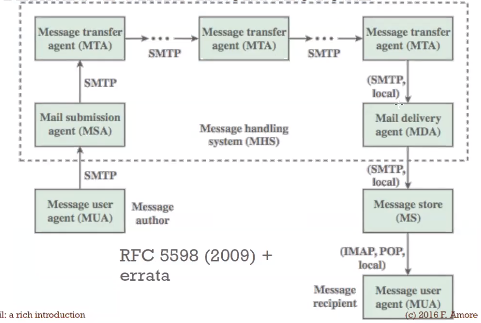
\includegraphics[scale=0.5]{./images/email_architecture.png}
\end{center}
In general, the way emails are transferred on the Internet follows the concept of the \textbf{store-and-forward model}. This means that, every time a MTA needs to send a message to the next one, it first stores the message locally and then forward the message to the next one waiting for a confirmation of the recipient (only at that point can delete the local message if needed). This enables one of the main characteristics of the system, which is the fact of being asynchronous. Typically an email is made up of three components :
\begin{itemize}
\item \textbf{message envelope} : it's used by MTAs to correctly relate the message from the sender MTA to the recipient MTA.
\item \textbf{message header} : where we write who is sending the email, who is the recipient, i.e. they are meta information. In particular, it's structured into fields such as From, To, CC, Subject, Date and other information about the email. It's separated from the message body by a blank line.
\item \textbf{message body} : it's the text of the message that we want to send, typically unstructured.
\end{itemize}
Each message has exactly one header, which is structured into fields. These fields are structured with name and value that are separated by a double column. There is also a possibility to define multi-line header fields. There are mandatory header fields such as :
\begin{itemize}
\item \textbf{From} : it's the sender email address.
\item \textbf{Date} : it's the local time and date when the message was sent.
\item \textbf{Message-ID} : it's an automatically generated field by the sender, to uniquely identify the message.
\item \textbf{In-Reply-To} : it's a message-ID that represents a link to a previous message to which the current message is a response to.
\item \textbf{To} : it's the recipient email address.
\end{itemize}
Other common header fields are the following :
\begin{itemize}
\item \textbf{Subject} : it's a brief summary of the topic of the message.
\item \textbf{Bcc} : with this option we can add addresses to the SMTP delivery list but they will not appear in the message data, i.e. they are invisible to other recipients.
\item \textbf{Cc} : it's similar to the previous field, but in this case all the addresses in the SMTP delivery list are listed in the message data. 
\item \textbf{Content-Type} : it's the field that allows the use of extensions like MIME type.
\item \textbf{References} : it's similar to the In-Reply-To field, but contains a list of previous messages. It should be coherent with In-Reply-To field.
\item \textbf{Reply-To} : it's mainly used to indicate to the client what to do if the user will click the reply button.
\item \textbf{Sender} : it's the address of the actual sender acting on behalf of the author listed in the From field (list manager, secretary, etc).
\end{itemize}
Together with the headers that we talked about, SMTP defines a lot of trace information that are included in the message as it's relayed toward the destination, which are also saved in the header using the following two fields :
\begin{itemize}
\item \textbf{Received} : it's populated every time the message is received by a MTA, with information about the MTA itself such as location, IP address, domain, etc. In this way we can rebuild the history of the message through the various relaying steps in its path toward the destination.
\item \textbf{Return-Path} : it's a field defined by the final MTA.
\end{itemize}
\subsection{MIME}
Another standard often used in email system is MIME (Multipurpose Internet Mail Extensions), but it's also used in the web for other reasons. It's a standard that explain us how to encode complex content in more simpler containers. It allows to include : text in character sets other than ASCII, non-text attachments, message bodies with multiple parts and header information in non-ASCII character sets. MIME is one of the things that changed the usage of Internet in the last 20 years. Now, the question is how does MIME works ? The idea is the following one : when the user want to send a message through the email system that contains some information that are not in the ASCII character set, the client encodes this information using MIME in a transparent way. First it analyze the content that is provided by the user, checks how each part of the content should be encoded and set up a MIME compliant message with the correct encoding of each part. Then this MIME encoded message is fully expressed using only 7 bit ASCII encoding and then it can be sent via the email system. At the other end of the email system when the message is received, the client of the receiver apply the opposite process, decoding the MIME content and correctly rendering the content of the message.
\begin{center}
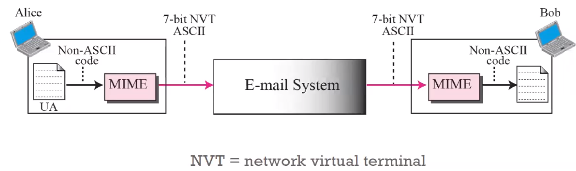
\includegraphics[scale=0.5]{./images/mime_schema.png}
\end{center}
The important point is that the MIME encoding of the message body is completely transparent to the email system, because MIME provides a way to encode and decode this content at the endpoint, and everything is completely transparent to the email system since it never look at the message content. The kind of encoding used for MIME is defined through MIME headers which contains the version information, the type of the content that will be provided by the email body and other meta data such as encoding type, content-id and content-description. Some of the most common MIME types are \textit{text/plain} for plain text data, \textit{text/html} for html content, etc. If for example we consider a jpeg image, this is not basic ASCII, how can we represent this richer content within a part of the body with the correct content type, but still sticking with the standard 7 bit ASCII ? For this reason, MIME defines several content transfer encoding methods : 7 bit, 8 bit, binary, base64 and quoted-printable encoding. Base64 is the standard way to encode non textual content in MIME messages. The idea is that through base64 we start from a binary content and obtain as target a string that is limited to $A-Z, a-z, 0-9,+, /$ character set. Typically the Non-ASCII data are divided in group of 8 bits, and combined in a certain number of 6 bit chunks. After that, each of them is interpreted as a number that is used as an index towards the 7 bit ASCII table. The good point is that having chunks of 6 bits we can range from $0$ up to $63$, which correctly maps to a 7 bit ASCII table. Considering that we are splitting and combining back the original stream of data, we may end up with some missing characters. So base64 encoded data typically may end with one or two symbols (they are equal symbols). The first advantage of this encoding scheme is for sure its simplicity to implement and apply to any kind of byte encoded content. Another good point is that, once we have the possible indexes that comes up from the various combinations of 6 bit that we use as chunk size, we can easily build a base64 converting table, such that an algorithm can just work as an iteration on the byte stream that looks up characters that make up the encoded stream. The disadvantage is that we are just using a subset of the 7 bit ASCII character set, and this means that there is some space that is wasted in the encoding. The encoding is obviously not space efficient. Another option is called quoted-printable encoding, where any 8 bit byte value may be encoded with three characters : an equal sign followed by two hexadecimal digits representing the byte's numerical value; instead any non 8 bit byte values are ASCII chars from $33$ to $126$, excluding $61$ (equal sign). It's extremely inefficient, because we encode 8 bits with 21 bits. However, its main advantage is that if for some reason the endpoint that receive the message is not able to decode quoted-printable encoding, the text is still mostly readable.
\subsection{Unwanted email messages}
Lets try to understand which are the weaknesses of these standards and how they are used to send unwanted email that typically comes with the name of \textbf{SPAM}. They are used to advertise any kind of merchandise. It's also used for a different goal such as performing some actions to take control of part or the full machine that the user is actually connected with. Another source of spam are called \textbf{e-mail chain letters}, with which induces you to fraud other people to get some benefit. Another characteristic of spam is the quality of the message itself. For example a message with a very low text quality, can be easily classified as spam. However, the low quality is something that is disappearing quite quickly. Naturally the spammers main goal is to spread the malware, in order to control computers for future attacks, steal sensitive information, and so on so forth.
\subsection{Basic email nonalogue}
We report a brief list of suggestions to follow when using the email system.
\begin{itemize}
\item Disable html message or, at least, disable download of remote images
\item Don't click links, since we could redirect us to bad web sites containing malware
\item Don't open unknown attachments since they may contain malware
\item activate local anti-spam filter
\item Don't participate with chain letters
\item Protect and respect privacy of other recipients
\item Even if non-Windows user, activate antivirus for protecting your recipients
\item Don't provide your personal data
\item Don't click "delete me" link.
\end{itemize}
\subsection{SMTP extensions}
We know that there are some pitfalls in the email system. For this reasons, there are other solutions that complements SMTP in order to provide some security features. In particular we will talk about three of them : \textbf{SPF}, \textbf{DKIM} and \textbf{VBR}.

\subsubsection{Sender Policy Framework}
One big problems with emails is the fact that the body and the envelope of the email are somewhat separated entities. The body of the email is built in the client that creates the email, while the email envelope is forged on the server through the interaction between the client and the server. Furthermore, in the SMTP protocol no where is written that it should be a coherence between some of the headers present in the email and what is written in the envelope (e.g. From field in the body equal to the From field in the envelope). SPF is a standard to solve this problem from a specific standpoint. In particular, SPF protects the sender address only in the envelope, it doesn't care about the From field in the email header. It allows the administration of the domain through which an email is sent, to define some policies about who could send emails through that server. So, receivers verifying the SPF records may reject message from unauthorized sources before receiving the body of the message. The nice point is that this will happen only looking at the email envelope; so is the server itself that can do this check and possibly reject the message, without the client even receiving the body. When the server accept the sender, it receives through the SMTP interaction the list of recipients and the message body. At that point it's expected to insert in the message header a field called Return-Path, in which it needs to save the sender address as is reported in the envelope. This means that this Return-Path may or may not correspond to the From header in the message. If the two are the same typically the message is fine; if they are different, SPF does not necessary mark the message as spam. We want to underline that SPF doesn't enforce the correspondence between these headers; they should match, but not in all cases. Naturally SPF by doing checks only on the sender field in the envelope has some limitations : keep the SPF record update as companies change service providers and add mail streams is difficult. Another bad point is that given that SPF is not perfect, the check on SPF it's just one among several checks that email servers typically do to avoid spam to reach a target email. Another important point is that typically SPF breaks whenever a message is forwarded, because the forwarder address could not be whitelisted in the DNS text record and at that point the SPF check will fail. The last point is that SPF makes no check on the From header contained in a message that wrt SPF can be easily spoofed.

\subsubsection{DKIM}
Given that SPF only works on the email envelope, someone started to think about introducing a different solution to take care of the security of the message headers called \textbf{DomainKeys Identified Mail}. It specifies how some parts of the message can be cryptographically signed in order to avoid their content to be tampered by other people (MITM attack or non-intended source creates a fake message with false source information). The idea of DKIM is that when you receive a DKIM signed message, as a recipient you can verify the signature that is contained in the message by querying the domain dns server for the information needed to check that signature. This is important because the rational behind DKIM is that it links the content of the email that is signed, with an information that is obtainable through a query to the dns of the sender. So the idea is that the two will be coherent only if they originates from the same person (domain administrator) or people that the domain administrator allows to use this kind of feature. A classic deployment of DKIM works in the following way
\begin{center}
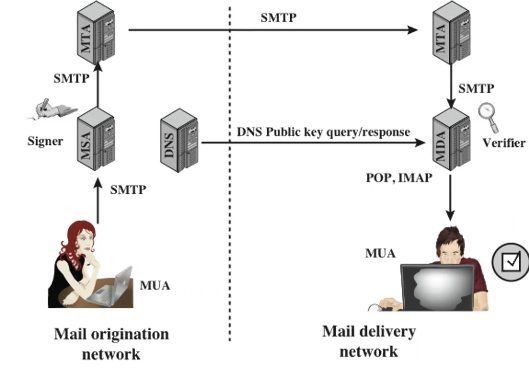
\includegraphics[scale=0.35]{./images/dkim_deployment.png}
\end{center}
First of all we have the origin of the email through a client. The client connects through SMTP with the server, but the call is intercepted by a \textbf{message signing authority (MSA)} that provides all the features to correctly sign the content of the message. Then the MTA through the SMTP protocol delivers the message to the endpoint to the server on the recipient side and this goes through a MDA, which checks through a query to the dns system if the signed content of the message is verified or not. If it's verified the MDA delivers the message to the end user. However, there is a practical problem when this protocol is widely deployed on the web. The email may pass through several servers, that typically may decide to add information in the headers of the email to keep track of what happened to the message on its path to the destination. Some of this changes can easily break the signature, because even if we just include the headers that are not expected to change in the path, some servers may include processing features that will alter the content of those headers. To avoid this kind of problem DKIM include a mechanism called \textbf{canonicalization}, through which it's possible to tell to the recipient if he needs to be strict in the checking of the signature of if he can perform a relaxed check. In this latter case, before applying the hash function to the headers, the recipient will for example make all the headers lowercase, remove all extra spaces, etc. Typically the relaxed checks says from easy rejection due to somewhat changes in the header that don't represent real mangling with the message content. Another detail that is important is represented by \textbf{selectors}. They allow to multiplex several private/public key pairs for the same domain, while providing a way for the recipient to check the correct one.

\subsubsection{DMARC}
In order to make SPF and DKIM work together to guarantee us that no one will make a wrong use of the available email services, we can use a standard called \textbf{Domain-based Message Authentication, Reporting, and Conformance (DMARC)}. It's interesting because it's not really a technical standard, but it's more or less a standard defining a process to integrate SPF and DKIM within a set of best practices that allow to make the best of them. In particular, DMARC allows organization to publicly declare policies through which they can define which kind of practices they put in place to guarantee email authentication. Furthermore, it provides instructions to the recipients to enforce these policies and report possible misuse. In particular, the domain owner publish its practices, he tell what to do when there is a failure with an authentication check and enables reporting. How does DMARC works ?
\begin{enumerate}
\item The first thing you need to do in order to use DMARC is to publish a policy. The publishing of a policy is performed through your dns records and again it uses the TXT records embedding some information for DMARC associated with that specific domain. In particular, it uses a TXT record that starts with $\_dmarc.$ followed by the name of your domain.
\item When the recipient server receives an incoming email containing the DMARC headers, it performs first of all a dns query to check the policies of the sender. This query is based on the domain declared in the From field of the email. Next, it checks three aspects of the message : checks if the message's DKIM is valid or not, checks if the message come from IP addresses allowed by domain's SPF record and checks if the message headers show proper domain alignment. The domain alignment is an aspect that is specific of DMARC. It expands what SPF and DKIM actually already do, and it checks if various elements in the domain headers match the domain declared in the From field. In particular, for SPF it checks if the domain in the From field correspond to the domain indicated in the Return-Path field; for DKIM it checks if the domain in the From field correspond to the domain listed in the d field of the DKIM header.
\item With this information, the recipient server is ready to apply the sending domain's DMARC policy to decide whether accept, reject or flag the email message.
\item Finally, the recipient server will report the outcome to the sending domain owner. In particular, there are two formats of DMARC reports :
\begin{itemize}
\item \textbf{Aggregate reports} : they represent statistical data on how many spoofed email for those domain has been received on a total of emails, or stuff like that. They are sent periodically, and not immediately sent at the reception of an email.
\item \textbf{Forensic reports} : they represent information about the checks the recipient server has performed and why they failed, but it has to include in the reports the original email that failed the checks. It allows the sender to perform some debugging for example to see if there is a problem with the DMARC configuration  and it also allow the owner of the sender domain to check if spoofing happens with specific patterns and possibly track down the origin of those spoofed emails and take some mitigations for that.
\end{itemize}
\end{enumerate}
In particular a DMARC record has the following fields :
\begin{itemize}
\item \textbf{v} : it specifies the DMARC version to be used.
\item \textbf{p} : it specifies which are the standard policies that needs to be applied to emails. It can assume one of the following three different choices : \textbf{none} for treat the mail the same as it would be without any DMARC validation, \textbf{quarantine} for accepting the mail, but place it somewhere other than the recipient's inbox, and \textbf{reject} in order to reject the message.
\item \textbf{rua} : it's the mail address to which aggregate reports should be sent
\item \textbf{ruf} : it's the mail address to which forensics reports should be sent
\item \textbf{pct} : it specifies the percentage of mail to which the domain owner would like to have its policy applied (it's an optional parameter).
\end{itemize}
The outcomes from protocol checks are reported in the mail headers.

\subsubsection{VBR}
Another protocol that we want to talk about is called \textbf{Vouch By Reference (VBR)}. It takes a completely different approach that is still orthogonal to SPF and DKIM, and in fact it can be used together with these solutions. In particular, VBR allows the implementation of sender certification by third-party entities. The idea is that it allows providers to independently certify the reputation of senders by checking the domain name. When you send an email using VBR, you use the standard DKIM protocol to sign the email, and then include in the signature a VBR-info field, which includes several information such as the domain name that is going to be certified, which content of the message is allowed to deliver and a list of one or more vouching services, that is the domain names of the services that vouch for the sender for that kind of content. At the receiver side, after checking the correctness of the DKIM or SPF headers, the software may possibly double check the VBR info by performing dns queries on the domain name of the services included in the VBR-info field. In particular, it will look for entries of type TXT that have this structure \textit{domain name.\_vouching service}. If VBR is checked at recipient side, the outcome of this check will be included in the Authentication Results field in the message header.

\subsection{Basic email analysis}
\textbf{Email spoofing} means altering some or majority of the elements that are present in the email header. The spoofer do that for hiding its real identity, since most of the content of spoofed emails is typically malicious in some form. How can the content of the email headers be spoofed ? At least for the sender address this is really simple, since SMTP doesn't include any authentication for senders. How do we check for spoofing ? Actually there are no deterministic approaches for doing that. For this reason, we can follow some guidelines that helps to understand if the message has been spoofed or not. A good starting point to do that is to analyze the complete message (full header + body), checking the From, Return-Path, Reply-To and Received header fields. In particular, in order to implement a secure email service we need :
\begin{itemize}
\item \textbf{confidentiality} : protection of the content from disclosure
\item \textbf{authentication} of the sender of the message
\item \textbf{message integrity} : protection from alterations
\item \textbf{non-repudiation} of origin : protection from denial by sender. 
\end{itemize}
\subsection{PGP}
\textbf{Pretty Good Privacy (PGP)} is an open protocol with proprietary and publicly open implementation. The basic point about PGP is that it was designed by incapsulating the usage of cryptographic primitives inside the email usage process. PGP is constituted by two main functionalities :

\paragraph{PGP Authentication} When the sender creates the message, computes its hash and uses a private key to sign the hash. Next, the message and the signature are put together to form the signed message. On the recipient side, the message signature is decoded using the sender public key and the result is compared with the hash of the message itself. If the two hashes are coherent this means that the message has not been tampered.
\begin{center}
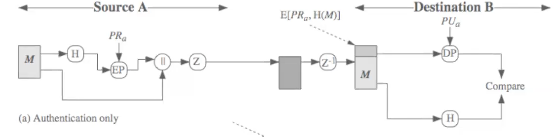
\includegraphics[scale=0.5]{./images/pgp_authentication.png}
\end{center}

\paragraph{PGP Confidentiality} First the message is compressed and encrypted by the sender using a symmetric key called \textbf{session key}. Next, the session key is encrypted using RSA with the recipient public key. Next, the encrypted session key and encrypted message are sent together. The recipient takes the encrypted session key and decodes it using its own private key, obtaining the session key, that will be used to decode the original message.
\begin{center}
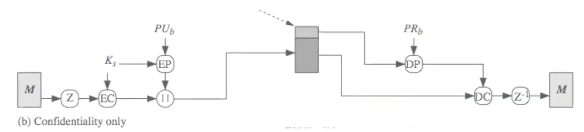
\includegraphics[scale=0.5]{./images/pgp_confidentiality.png}
\end{center}
Of course these functionalities can be used together (confidentiality \& authentication). As previously mentioned, PGP uses a compression function to reduce the size of messages, typically before the encryption phase. In this way it's possible to store uncompressed message and signature for later verification, because the point is that compression algorithm may introduce some non determinism. When we use PGP for sending binary data, it will encodes such data into printable ASCII characters using Base64 encoding. Session keys that are used for encode messages are built randomly for each encryption pass, and the implementation is typically based on a $256$ bit buffer which contains random bits. This buffer is updated every time you press a key interacting with PGP. It register the period of time between two keystrokes, plus the value of the keystroke itself, and use this information as a key to encrypt again the content of that buffer. In PGP you may possible own as a user more than one public/private keys pair, in order to send different kind of messages or to interact with a different group of people. To identify which couple has been used to encrypt a message, the message is sent including the public key plus the ID of the key identifier of that couple of key. The key identifier is simply extracted from the least significant $64$ bits of the public key. In PGP implementation each user maintains through its client two \textbf{key rings} : the public key ring contains all the public keys of other PGP users known to this user, indexed by the key ID, the private key rings contains the public/private key pairs used by the current user and they are indexed by the key ID and encrypted using some passphrase. Now the question is, how do we manage these keys ? In PGP every user represent its own Certification Authority (CA), which is able to create all the public/private key pairs needed. The main disadvantage is that this removes the so called assumption on the presence of a trusted third party, that makes this approach usable for example for signing digital certificates. Instead, PGP rely on the concept of \textbf{web of trust}. The idea is that when you start using PGP, you need to get the recipients public keys, and then start to trust these recipients and they will trust you. This mechanism will iteratively creates a web of trust, where keys brings with them a sort of certificate of trust that says that those keys have been trusted by other users and this should increase the possibility that they are also trusted by someone else that have never seen before those keys. For this reason, key rings includes trust indicators in their data structure. This web of trust somewhat is a vision that looks at reality where the trust is something that emerges from a decentralized fault-tolerance web of confidence.

\subsection{ARC}
The \textbf{Authenticated Received Chain (ARC)} protocol proposes a solution to overcome the problems that we may have using SPF and DKIM. In particular, instead of enforcing security only between the sender and receiver, it allows to completely track security checks through the full chain of relays that are encountered while an email is in transit. The reasons why messages can fail DMARC policies checks are for examples : strict policies, the message pass through some indirect mail flow such as mailing list, attachments removal, etc. To overcome these problems people started to think about ARC trying to sketch out which are the main design choices for the definition of this new protocol. In particular, the main design decisions are the following :
\begin{itemize}
\item the originator of the message doesn't need to make any change to the message itself
\item convey Authentication-Results content intact from the first ARC intermediary forward
\item allow for multiple hops in the indirect mail flow
\item ARC headers can be verified at each hop
\item work at Internet scale
\item we need to make ARC as independent as possible from DMARC.
\end{itemize}
The idea of ARC on the recipient side is that the receiving endpoint should perform the standard DMARC checks. But if a failure is result of these checks, then optionally the receiver may possibly look for the presence of ARC headers, and use them to perform a more extensive check. If this extensive check give us a negative result then the server may possibly decide to locally override for that message the final decision for the DMARC policy. How does the ARC headers checks actually works ? Through the ARC header the final recipient need to be able to look at the value of the original Authentication-Results field as it was created by the first hop in the mail forwarding chain, and then checks the authenticity of all the intermediate steps that have been traveled through by the email from that first step up to the recipient point. So, the recipient will be able to validate the entire chain. Thus an intact ARC chain provides to the recipient the following information : it gives DKIM, DMARC and SPF results as they have been seen by the first hop in the mail forwarding chain. Then it provides signatures that show that these results were actually not tampered with someone else. Finally, signatures from participating intermediaries can be linked to their domain name to prove that they are actually what they pretend to be. However, this doesn't prevent intermediaries to alter the message content. The main point of ARC is that such alterations can be done only with attribution, with which we are able to identify who did such changes in the chain. ARC doesn't provide us a solution for any problem. For example ARC doesn't tell us how much trustable is the message sender or the intermediaries, it only provides us information of what they did with that message. It says nothing about the content of the message and what has been added by the intermediaries to the content itself. ARC introduces the following header fields :
\begin{itemize}
\item \textbf{ARC-Authentication-Results (AAR)} : it's an archived copy of the Authentication-Results as it has been seen by the first hop. Each intermediary will performs the checks locally. They will give rise to several AAR headers that will be relayed up to the final recipient. Given that they need to be ordered for the final recipient to correctly interpret their content and the evolution of these checks through out the full mail forwarding chain, the AAR header also include a special tag $i$ that contains a sequence number. The only Authentication-Results field that will not be archived in AAR header will be the one that is calculated on the final hop, i.e. the one computed by the recipient.
\item \textbf{ARC-Seal (AS)} : it's a header that includes a few tags that are needed to understand how ARC should work, and a DKIM style signature of any preceding headers. It's built like an incremental seal that provide a proof of the fact that all the ARC headers including AMS and AAR headers that are included in a message have been correctly created and have not been altered during the travel of the message through out the forwarding chain.
\item \textbf{ARC-Message-Signature (AMS)} : it's a modified DKIM signature.
\end{itemize}
The order of insertion is that first we have the AAR which are created with a simple copy of the Authentication-Results field, then the AMS and finally the AS. To summarize the ARC benefits for sender/intermediary are the following : it allows intermediaries to continue and/or resume traditional From semantics, message modifications, allows more senders to adopt strict DMARC policies, and improves overall deliverability. While the ARC benefits for the receiver are the following : less stress for enforcing DMARC policies, allows more mailbox providers to publish strict DMARC policies on their customer-facing domains and we have more data for reputation systems.

\subsection{S/MIME}
The authors of \textbf{S/MIME} protocol took all the approaches defined in PGP for signing and encrypting emails, and simply integrated them with a standard digital certificate based approach to trust. S/MIME is a widely used protocol for sending and receiving emails in a secure fashion, and its name comes from the fact that it somewhat extend the standard MIME protocol for encapsulating different kind of content in a single document, and it adds MIME types that are used on purpose to handle security mail content. Furthermore, it also adds some indication on how it implements email integrity and confidentiality. We can see that email signatures are handled exactly as in PGP
\begin{center}
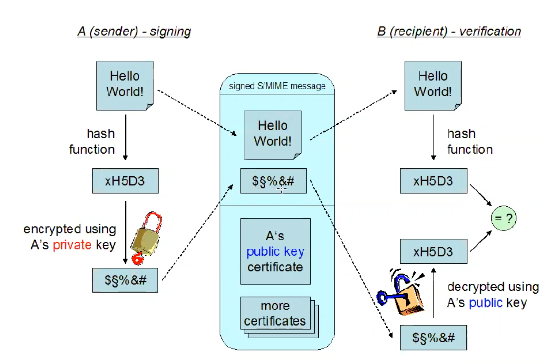
\includegraphics[scale=0.45]{./images/smime_schema.png}
\end{center}
The original message is passed through a hash function in order to provide a digest, which in turn it's signed using the sender private key. Then the original message and the signature are embedded in a S/MIME message. Differently from PGP, the message typically includes the public certificate of the sender and may possibly include other certificates that are needed to correctly enforce the trust upon this public key certificate. On the recipient side, we have the classic approach used in PGP, i.e. the recipient computes the digest of the original message, decrypt the signature using the sender public key extracted from the sender public key certificate, and checks if the result matches the digest previously computed. When we move to encryption, it's performed exactly in the same functional way, but using X.509 standard certificates. A random session key is chosen on sender side, it's encrypted using the recipient public key and then the original message is encrypted using that session key. Both the encrypted message and encrypted session key are encapsulated in a S/MIME message plus the sender public key certificate. Then on the recipient side, the opposite approach is used to decrypt the message as in PGP but for the presence of certificates. The real strong difference between PGP and S/MIME lies in how the identity of sender and recipient is handled by the protocol.

\subsection{How PEC works}
A possible approach to implement a mechanism on top of the email service to include beyond security functionalities also tracing functionalities that allows to trace what happens to the emails and make these traces visible both to the sender and receiver goes under the name of \textbf{Posta Elettronica Certificata (PEC)}. It works as follow : the sender wants to send an email to the receiver but he wants also to have a confirmation about the steps performed to manage this email in its travel from himself to the receiver. It's mainly based on the usage of S/MIME, plus a set of procedures that are needed to create certified timestamps about what is happening to the email. In particular, the sender creates an email and ask its service provider to deliver such email to the receiver. The provider at this point only enforce the authentication from the sender, i.e. it checks if the sender is actually what he's pretending to be and the content of the headers in the email are coherent with the digital identity of the sender. Once all these checks are ok, the provider sends back to the sender a certificate, which contains information about such checks and that the email has been taken in custody by itself. Next, the provider will take the content of the email and encapsulate that email in an envelope that is signed by itself. The envelope is then sent from the sender provider to the receiver provider through a reception point. The receiver provider checks if the signatures in the envelope are correct, and if it doesn't see any problem with the email, it will take into custody the email, and will send to the original sender a new certificate that attest the fact that he received the email from the sender provider with a specific timestamp and that he's now going to deliver the message to the receiver inbox. At this point, the receiver provider access the receiver inbox and place the message in it. When this happens, a new message will be sent to the sender saying "now the message is in the receiver inbox". In this way we have an email that is signed with a signed timestamp, and they are legally usable to attest the fact that an email was correctly delivered to a given recipient.